\chapter{Experiment}
\label{exp}
\begin{multicols*}{2}

	\section{Introduction}
	Here I will give a brief overview of the experiments that I will have conducted, the variations that they have between them, and why I chose those variations.

	\section{Experiments}
		\subsection{Control - Standard Euclidean Geometry}
		Here I will talk about the results from the control experiment, which will give a good baseline as to the level of immersion a user would have in the system when subject to standard Euclidean geometry.

		\subsection{Mix - Euclidean $\rightarrow$ Non-Euclidean}
		Here I will talk about results specific to the experiment where the user starts off in a standard Euclidean world, but where the world switches to non-Euclidean spaces towards the end of their path.

		\subsection{Mix - Non-Euclidean $\rightarrow$ Euclidean}
		Here I will talk about results specific to the experiment where the user starts off in a non-Euclidean world, but switches to use regular Euclidean space towards the end of their path.

		\subsection{Non-Euclidean}
		Here I will talk about the results from the experiment where the user will be subject to non-Euclidean space for the duration of the experiment.

	\section{Summary}
	Here I will be evaluating the results of the experiments, covering any trends that appeared between the various experiments, discussing potential impacts from the results, as well as covering any additional notes that were provided about the experiments from the participants which weren't directly related to the specific experiment they were part of.

\end{multicols*}

	\begin{figure}
		\label{exp:fig:standard_immersion}
		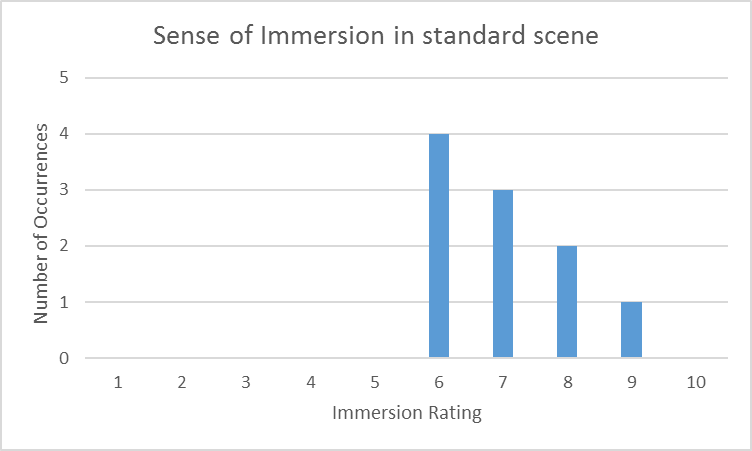
\includegraphics[width=0.7\textwidth]{Images/Standard_Immersion}
		\centering
		\caption{Immersion rating in standard geometry test scene}
	\end{figure}

	\begin{figure}
		\label{exp:fig:standard_comfort}
		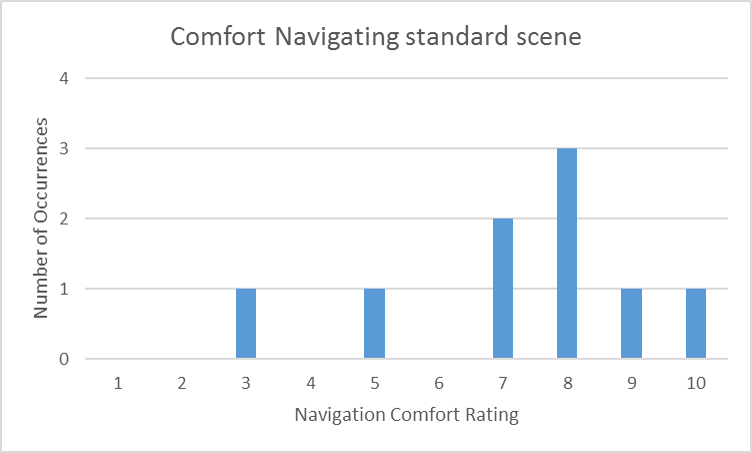
\includegraphics[width=0.7\textwidth]{Images/Standard_Comfort}
		\centering
		\caption{Navigation Comfort rating in standard geometry test scene}
	\end{figure}

	\begin{figure}
		\label{exp:fig:standard_relation}
		\includegraphics[width=0.7\textwidth]{Images/Standard_Relation}
		\centering
		\caption{Relation between sense of immersion and navigation comfort in standard geometry test scene}
	\end{figure}

	\begin{figure}
		\label{exp:fig:ne_immersion}
		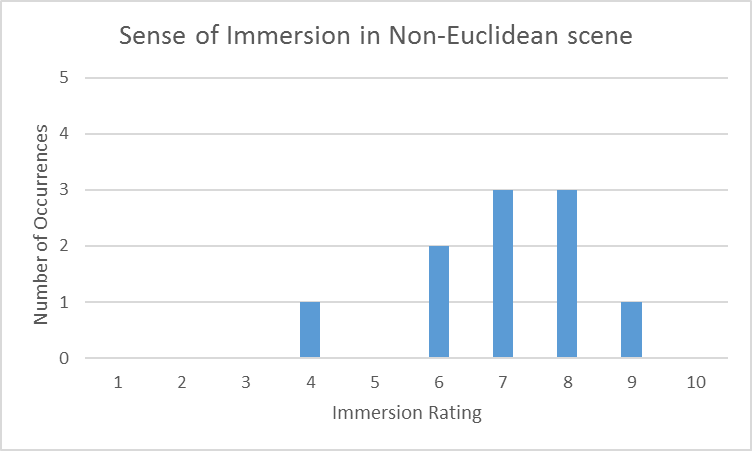
\includegraphics[width=0.7\textwidth]{Images/NE_Immersion}
		\centering
		\caption{Immersion rating in Non-Euclidean geometry test scene}
	\end{figure}

	\begin{figure}
		\label{exp:fig:ne_comfort}
		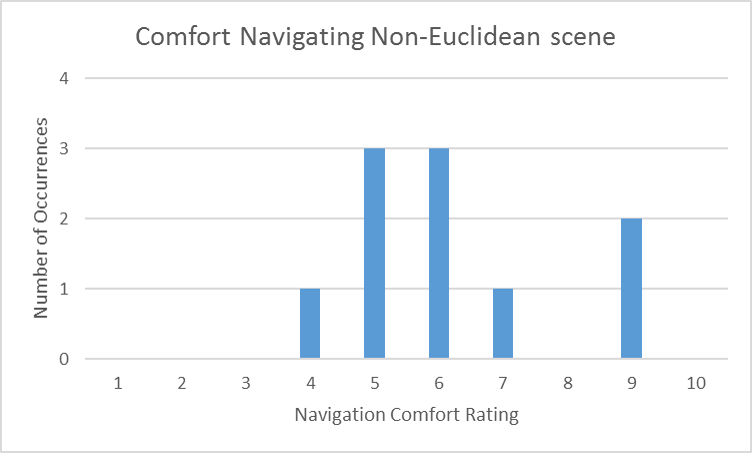
\includegraphics[width=0.7\textwidth]{Images/NE_Comfort}
		\centering
		\caption{Navigation Comfort rating in Non-Euclidean geometry test scene}
	\end{figure}

	\begin{figure}
		\label{exp:fig:ne_relation}
		\includegraphics[width=0.7\textwidth]{Images/NE_Relation}
		\centering
		\caption{Relation between sense of immersion and navigation comfort in Non-Euclidean geometry test scene}
	\end{figure}

	\begin{figure}
		\label{exp:fig:compare_immersion_exp1}
		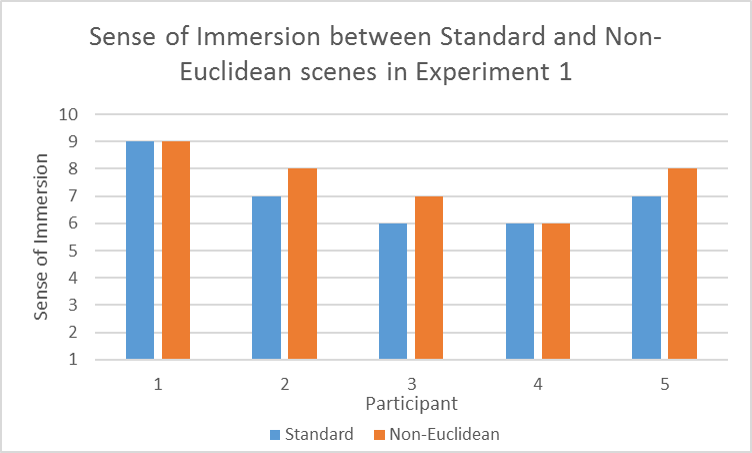
\includegraphics[width=0.7\textwidth]{Images/Compare_Immersion_Exp_1}
		\centering
		\caption{Comparison of participants sense of immersion in the two test scenes, from Experiment 1}
	\end{figure}

	\begin{figure}
		\label{exp:fig:compare_immersion_exp2}
		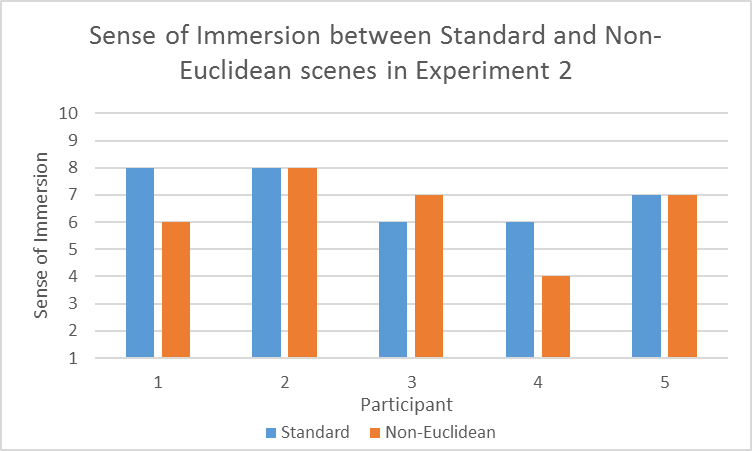
\includegraphics[width=0.7\textwidth]{Images/Compare_Immersion_Exp_2}
		\centering
		\caption{Comparison of participants sense of immersion in the two test scenes, from Experiment 2}
	\end{figure}

	\begin{figure}
		\label{exp:fig:compare_immersion_variation}
		\includegraphics[width=0.7\textwidth]{Images/Compare_Immersion_Variation}
		\centering
		\caption{Mean values, and variation of Range for Immersion in the two test scenes}
	\end{figure}

\begin{multicols*}{2}

\end{multicols*}